\documentclass[12pt]{article}
\newcommand{\ReportShortTitle}{Cá nhân -- Phạm Hùng Tiến}
\usepackage[a4paper,top=2.1cm,bottom=2.2cm,left=2.6cm,right=2.2cm,headheight=15pt]{geometry}
\usepackage{fontspec}
\setmainfont{Times New Roman}
\setsansfont{Arial}
\setmonofont{Menlo}[Scale=0.86]
\usepackage{microtype}
\usepackage{setspace}
\setstretch{1.22}
\usepackage{parskip}
\setlength{\parindent}{1.1cm}
\setlength{\parskip}{3pt}

\usepackage{xcolor}
% Hệ màu đơn sắc: chỉ dùng đen, trắng và các mức xám để in ấn chuyên nghiệp.
\definecolor{Primary}{gray}{0}
\definecolor{Secondary}{gray}{0}
\definecolor{Accent}{gray}{0.72}
\definecolor{SoftBlue}{gray}{0.94}
\definecolor{SoftGray}{gray}{0.97}
\definecolor{Success}{gray}{0}
\definecolor{Warning}{gray}{0}
% Màu chỉ dùng bên trong khối mã nguồn.
\definecolor{CodeKeyword}{HTML}{1F4E79}
\definecolor{CodeComment}{HTML}{3F6B45}
\definecolor{CodeString}{HTML}{8A4B08}

\usepackage{graphicx}
\usepackage{booktabs}
\usepackage{longtable}
\usepackage{tabularx}
\usepackage{array}
\usepackage{makecell}
\usepackage{multirow}
\usepackage{enumitem}
\usepackage{amsmath,amssymb}
\usepackage{tikz}
\usetikzlibrary{arrows.meta,positioning,shapes.geometric,fit}
\usepackage[most]{tcolorbox}
\usepackage{listings}
\usepackage{needspace}
\renewcommand{\lstlistingname}{Đoạn mã}
\renewcommand{\lstlistlistingname}{Danh sách đoạn mã}
\renewcommand{\contentsname}{MỤC LỤC}
\usepackage{titlesec}
\usepackage{fancyhdr}
\usepackage{lastpage}
\usepackage{hyperref}
\hypersetup{colorlinks=true,linkcolor=Primary,urlcolor=Secondary,citecolor=Primary,pdfborder={0 0 0}}

\setlist[itemize]{leftmargin=1.2cm,itemsep=2pt,topsep=3pt}
\setlist[enumerate]{leftmargin=1.2cm,itemsep=2pt,topsep=3pt}
\renewcommand{\arraystretch}{1.25}
\newcolumntype{Y}{>{\raggedright\arraybackslash}X}
\newcolumntype{C}[1]{>{\centering\arraybackslash}p{#1}}
\newcolumntype{L}[1]{>{\raggedright\arraybackslash}p{#1}}

\titleformat{\section}{\Large\bfseries\color{Primary}}{\thesection.}{0.55em}{}
\titleformat{\subsection}{\large\bfseries\color{Secondary}}{\thesubsection.}{0.5em}{}
\titleformat{\subsubsection}{\normalsize\bfseries\color{Primary}}{\thesubsubsection.}{0.5em}{}
\titlespacing*{\section}{0pt}{16pt}{7pt}
\titlespacing*{\subsection}{0pt}{11pt}{5pt}

\pagestyle{fancy}
\fancyhf{}
\fancyhead[L]{\small\color{Primary}\textbf{ĐỒ ÁN ESP32-S3}}
\fancyhead[R]{\small\color{Secondary}\ReportShortTitle}
\fancyfoot[L]{\small Nhóm 3 thành viên}
\fancyfoot[R]{\small Trang \thepage/\pageref{LastPage}}
\renewcommand{\headrulewidth}{0.5pt}
\renewcommand{\footrulewidth}{0.4pt}

\newtcolorbox{summarybox}[1][Tóm tắt]{
  enhanced, breakable, colback=SoftBlue, colframe=Secondary,
  title=\textbf{#1}, coltitle=white, colbacktitle=Secondary,
  boxrule=0.7pt, arc=2mm, left=3mm, right=3mm, top=2mm, bottom=2mm
}
\newtcolorbox{evidencebox}[1][Minh chứng]{
  enhanced, breakable, colback=SoftGray, colframe=Primary,
  title=\textbf{#1}, coltitle=white, colbacktitle=Primary,
  boxrule=0.6pt, arc=1.5mm, left=3mm, right=3mm, top=2mm, bottom=2mm
}
\newtcolorbox{warningbox}[1][Lưu ý]{
  enhanced, breakable, colback=Accent!12, colframe=Warning,
  title=\textbf{#1}, coltitle=white, colbacktitle=Warning,
  boxrule=0.6pt, arc=1.5mm, left=3mm, right=3mm, top=2mm, bottom=2mm
}

\lstdefinestyle{firmware}{
  language=C++,
  basicstyle=\ttfamily\fontsize{8.35}{10.2}\selectfont,
  keywordstyle=\color{CodeKeyword}\bfseries,
  commentstyle=\color{CodeComment}\itshape,
  stringstyle=\color{CodeString},
  numbers=left,
  numberstyle=\sffamily\fontsize{6.8}{8.2}\selectfont\color{black!48},
  numbersep=9pt,
  frame=lines,
  framerule=0.45pt,
  rulecolor=\color{black!68},
  backgroundcolor=\color{white},
  framesep=5.5pt,
  breaklines=true,
  breakatwhitespace=false,
  breakindent=1.25em,
  columns=fullflexible,
  keepspaces=true,
  showstringspaces=false,
  tabsize=2,
  escapeinside={(*@}{@*)},
  xleftmargin=1.1em,
  xrightmargin=0.25em,
  framexleftmargin=1.0em,
  framexrightmargin=0.45em,
  aboveskip=9pt,
  belowskip=10pt,
  abovecaptionskip=6pt,
  belowcaptionskip=0pt,
  captionpos=b
}

% Chú thích tiếng Việt được render bằng XeLaTeX ngay trong khung mã.
\newcommand{\VNCodeComment}[1]{%
  \parbox[t]{0.93\linewidth}{%
    \raggedright\color{CodeComment}\sffamily\fontsize{7.7}{9.1}\selectfont\itshape
    \textcolor{CodeComment}{\textbf{//}}\enspace #1}%
}

\newcommand{\ProjectTitle}{THIẾT BỊ ĐEO THEO DÕI SỨC KHỎE, PHÁT HIỆN TÉ NGÃ VÀ ĐỊNH VỊ DÙNG ESP32-S3}
\newcommand{\GroupMembers}{Phạm Hùng Tiến -- Hồ Sĩ Phú -- Quách Gia Thịnh}
\newcommand{\ReportDate}{Tháng 8 năm 2026}
\newcommand{\RepositoryURL}{https://github.com/PhamHungTien/esp32-s3-health-monitor}
\newcommand{\RepositoryDisplay}{github.com/PhamHungTien/esp32-s3-health-monitor}
\newcommand{\UniversityName}{TRƯỜNG ĐẠI HỌC KHOA HỌC TỰ NHIÊN}
\newcommand{\UniversitySystem}{ĐẠI HỌC QUỐC GIA THÀNH PHỐ HỒ CHÍ MINH}
\newcommand{\FacultyName}{KHOA ĐIỆN TỬ -- VIỄN THÔNG}

\newcommand{\CoverInstitution}{%
  \centering
  
\includegraphics[height=2.8cm]{assets/branding/hcmus_logo_user.png}\par
  \vspace{0.2cm}
  {\sffamily\bfseries\small\color{Primary}\UniversitySystem\par}
  \vspace{2pt}
  {\sffamily\bfseries\fontsize{16}{20}\selectfont\color{Primary}\UniversityName\par}
  \vspace{3pt}
  {\sffamily\bfseries\large\color{Secondary}\FacultyName\par}
  \vspace{0.35cm}
  {\color{Primary}\rule{0.84\textwidth}{1.0pt}\par}
}

\newcommand{\CoverBands}{%
  \begin{tikzpicture}[remember picture,overlay]
    \fill[Primary] (current page.north west) rectangle ([yshift=-4.5mm]current page.north east);
    \fill[Secondary] (current page.south west) rectangle ([yshift=3mm]current page.south east);
  \end{tikzpicture}%
}

\newcommand{\CoverField}[2]{%
  \noindent
  \begin{minipage}[t]{0.35\linewidth}
    \raggedright\strut\sffamily\bfseries\color{Primary}#1
  \end{minipage}\hfill
  \begin{minipage}[t]{0.61\linewidth}
    \raggedright\strut\sffamily\color{black}#2
  \end{minipage}\par
}

\hypersetup{
  pdftitle={\ProjectTitle\space -- \ReportShortTitle},
  pdfauthor={\GroupMembers},
  pdfsubject={Báo cáo đồ án thiết bị theo dõi sức khỏe dùng ESP32-S3},
  pdfkeywords={ESP32-S3, MAX30102, OLED, IMU, GPS, nhịp tim, SpO2, té ngã}
}

\newcommand{\MakeReportCover}[4]{%
  \hypersetup{pageanchor=false}
  \begin{titlepage}
    \thispagestyle{empty}
    \centering
    \CoverBands
    \vspace*{0.05cm}
    \CoverInstitution
    \vspace{0.45cm}
    {\sffamily\bfseries\normalsize\color{Secondary} BÁO CÁO ĐỒ ÁN\par}
    \vspace{0.35cm}
    {\sffamily\bfseries\fontsize{18}{23}\selectfont\color{Primary}\ProjectTitle\par}
    \vspace{0.6cm}
    \begin{tcolorbox}[width=0.84\textwidth,colback=SoftBlue,colframe=Secondary,arc=1.8mm,boxrule=0.8pt,left=4mm,right=4mm,top=2.7mm,bottom=2.7mm]
      \centering{\sffamily\bfseries\normalsize\color{Secondary} #1\par}
    \end{tcolorbox}
    \vfill
    \begin{tcolorbox}[width=0.84\textwidth,colback=white,colframe=Primary!48,arc=1.2mm,boxrule=0.6pt,left=6mm,right=6mm,top=4.5mm,bottom=4.5mm]
      \raggedright
      \CoverField{Người thực hiện}{#2}
      \vspace{2.1mm}
      \CoverField{Mã số sinh viên}{#3}
      \vspace{2.1mm}
      \CoverField{Nhóm}{03 thành viên}
      \vspace{2.1mm}
      \CoverField{Phạm vi báo cáo}{#4}
    \end{tcolorbox}
    \vfill
    {\sffamily\footnotesize\color{Secondary}\GroupMembers\par}
    \vspace{0.2cm}
    {\sffamily\footnotesize\color{Primary}\textbf{Mã nguồn đồ án: }
      \href{\RepositoryURL}{\RepositoryDisplay}\par}
    \vspace{0.2cm}
    {\sffamily\bfseries\small\color{Primary}Thành phố Hồ Chí Minh, \ReportDate\par}
    \vspace{0.2cm}
  \end{titlepage}
  \hypersetup{pageanchor=true}
  \clearpage
}

\newcommand{\MakeGroupCover}[1]{%
  \hypersetup{pageanchor=false}
    \begin{titlepage}
    \thispagestyle{empty}
    \centering
    \CoverBands
    \vspace*{0.05cm}
    \CoverInstitution
    \vspace{0.45cm}
    {\sffamily\bfseries\normalsize\color{Secondary} BÁO CÁO ĐỒ ÁN\par}
    \vspace{0.35cm}
    {\sffamily\bfseries\fontsize{18}{23}\selectfont\color{Primary}\ProjectTitle\par}
    \vspace{0.6cm}
    \begin{tcolorbox}[width=0.84\textwidth,colback=SoftBlue,colframe=Secondary,arc=1.8mm,boxrule=0.8pt,left=4mm,right=4mm,top=2.7mm,bottom=2.7mm]
      \centering{\sffamily\bfseries\normalsize\color{Secondary} #1\par}
    \end{tcolorbox}
    \vfill
    \begin{tcolorbox}[width=0.84\textwidth,colback=white,colframe=Primary!48,arc=1.2mm,boxrule=0.6pt,left=6mm,right=6mm,top=4.5mm,bottom=4.5mm]
      \sffamily
      {\bfseries\color{Primary}THÀNH VIÊN THỰC HIỆN\par}
      \vspace{3mm}
      \begin{tabularx}{\linewidth}{C{1.1cm} Y C{3.0cm}}
        \toprule
        \textbf{STT} & \textbf{Họ và tên} & \textbf{MSSV}\\
        \midrule
        1 & Phạm Hùng Tiến & 24207043\\
        2 & Hồ Sĩ Phú & 24207101\\
        3 & Quách Gia Thịnh & 24207105\\
        \bottomrule
      \end{tabularx}
    \end{tcolorbox}
    \vfill
    {\sffamily\footnotesize\color{Primary}\textbf{Mã nguồn đồ án: }
      \href{\RepositoryURL}{\RepositoryDisplay}\par}
    \vspace{0.2cm}
    {\sffamily\bfseries\small\color{Primary}Thành phố Hồ Chí Minh, \ReportDate\par}
    \vspace{0.2cm}
  \end{titlepage}
  \hypersetup{pageanchor=true}
  \clearpage
}

\newcommand{\Code}[1]{\texttt{#1}}
\newcommand{\OK}{\textcolor{Success}{\textbf{Đạt}}}
\newcommand{\Implemented}{\textcolor{Secondary}{\textbf{Đã cài đặt}}}
\newcommand{\NeedTest}{\textcolor{Warning}{\textbf{Cần thử thêm}}}
\newcommand{\Pending}{\textcolor{Warning}{\textbf{Cần hiệu chuẩn}}}


\begin{document}
\MakeReportCover{BÁO CÁO CÔNG VIỆC CÁ NHÂN}{Phạm Hùng Tiến}{24207043}{Tích hợp hệ thống, giao tiếp I2C, hiển thị và quy trình nạp}

\begin{summarybox}[Nội dung phụ trách]
Trong đồ án, em phụ trách cấu hình ESP32-S3 N16R8, giao tiếp I2C, điều khiển OLED SSD1306, bố trí lịch chạy các cảm biến và kiểm tra hoạt động chung của thiết bị.
\end{summarybox}

\section{Mục tiêu công việc}

Mục tiêu của phần việc là bảo đảm các cảm biến, GPS và màn hình có thể chạy đồng thời trên ESP32-S3. Chương trình cần đọc dữ liệu liên tục, cập nhật màn hình đúng chu kỳ và vẫn giữ được kết nối khi một mô-đun được cắm lại.

\section{Công việc đã thực hiện}

\subsection{Thiết kế cấu hình phần cứng}

Em sử dụng cấu hình bo \textbf{ESP32-S3 N16R8}, flash 16 MB, PSRAM 8 MB và chế độ USB CDC khi khởi động. Bus I2C dùng GPIO8 làm SDA và GPIO9 làm SCL. Khi quét bus, chương trình nhận được OLED tại 0x3C, MAX30102 tại 0x57 và IMU tại 0x68. Cụm camera được tách khỏi bus vì các chân 8--9 trùng với tín hiệu camera của bo.

\begin{figure}[htbp]
  \centering
  \begin{minipage}[t]{0.48\textwidth}
    \centering
    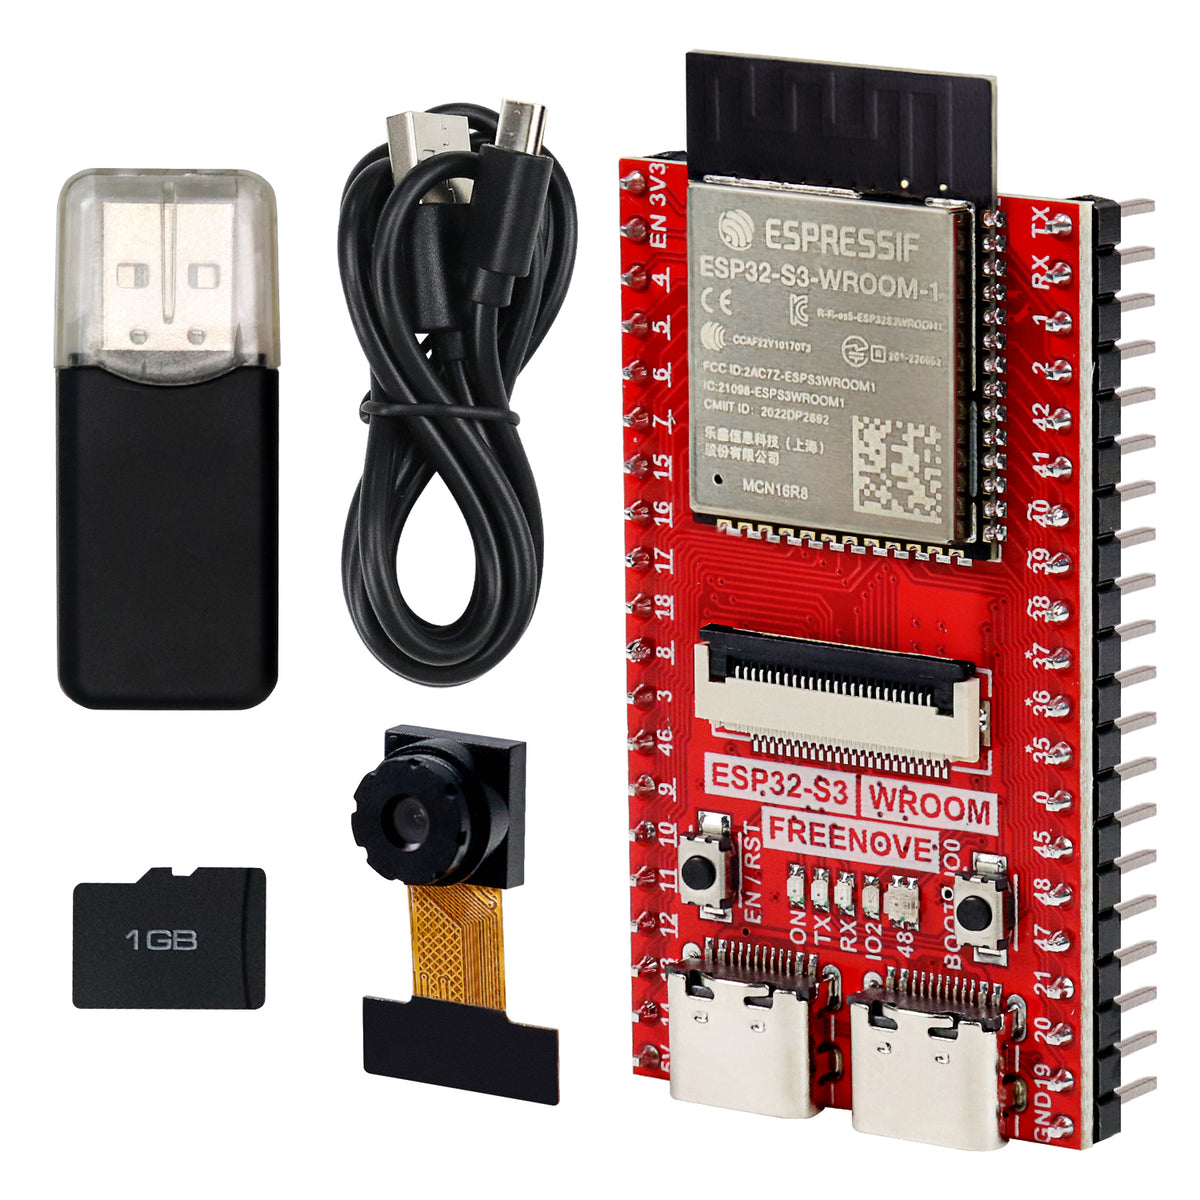
\includegraphics[width=0.92\linewidth,height=4.7cm,keepaspectratio]{assets/components/esp32s3_freenove.jpg}
    \\[2pt]\small (a) Bo Freenove ESP32-S3-WROOM N16R8.
  \end{minipage}\hfill
  \begin{minipage}[t]{0.48\textwidth}
    \centering
    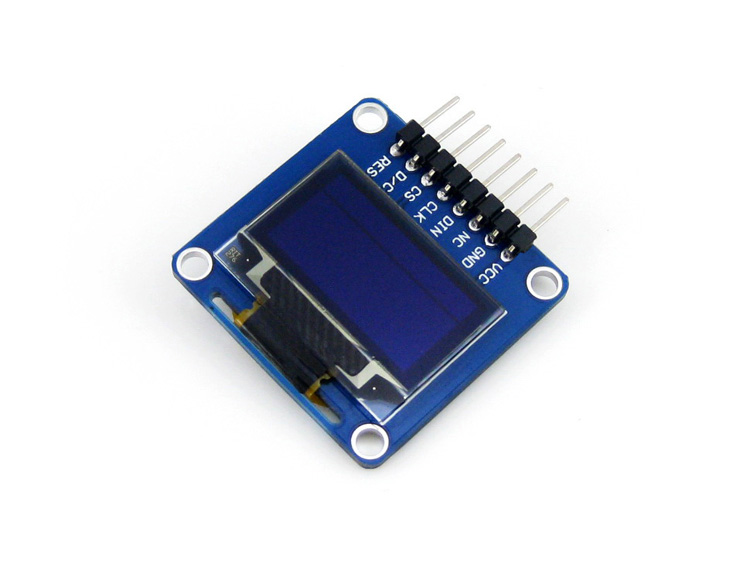
\includegraphics[width=0.92\linewidth,height=4.7cm,keepaspectratio,trim=110 30 110 30,clip]{assets/components/oled_ssd1306.jpg}
    \\[2pt]\small (b) Màn hình OLED SSD1306 0,96 inch tham chiếu.
  \end{minipage}
  \caption{Hai linh kiện thuộc phạm vi tích hợp và hiển thị. Nguồn ảnh: \href{https://store.freenove.com/products/fnk0085}{Freenove} và \href{https://www.waveshare.com/0.96inch-OLED-A.htm}{Waveshare}.}
  \label{fig:tien-hardware}
\end{figure}

\subsection{Giao tiếp I2C}

Em viết các thao tác đọc/ghi thanh ghi dựa trên \Code{Wire} có sẵn trong ESP32 Arduino Core, gồm phát START, gửi địa chỉ, ghi thanh ghi, repeated START và đọc nhiều byte. Giá trị trả về được dùng để nhận biết NACK hoặc thiếu dữ liệu. Chương trình thử kết nối lại sau mỗi hai giây nếu một thiết bị I2C bị rút ra.

Đoạn mã dưới đây là thao tác đọc một thanh ghi. Giá trị \Code{false} được truyền lên lớp gọi để mô-đun không tiếp tục sử dụng dữ liệu cũ khi bus báo lỗi.

\Needspace{0.26\textheight}
\begin{lstlisting}[style=firmware,caption={Đọc thanh ghi I2C và kiểm tra lỗi truyền}]
(*@\VNCodeComment{Khai báo hàm đọc một thanh ghi; địa chỉ thiết bị và địa chỉ thanh ghi là đầu vào, còn byte đọc được trả qua biến tham chiếu.}@*)
bool I2C_ReadRegister(uint8_t address, uint8_t reg, uint8_t &value) {
(*@\VNCodeComment{Bắt đầu một giao dịch I2C với thiết bị có địa chỉ đã truyền vào.}@*)
  Wire.beginTransmission(address);
(*@\VNCodeComment{Gửi địa chỉ thanh ghi cần đọc vào bộ đệm truyền của bus.}@*)
  Wire.write(reg);
(*@\VNCodeComment{Phát repeated START thay vì STOP; nếu thiết bị trả NACK thì kết thúc hàm với trạng thái lỗi.}@*)
  if (Wire.endTransmission(false) != 0) return false;
(*@\VNCodeComment{Yêu cầu đúng một byte từ thiết bị; số byte nhận khác một được xem là lỗi truyền.}@*)
  if (Wire.requestFrom(address, (uint8_t)1) != 1) return false;
(*@\VNCodeComment{Lấy byte đang chờ trong bộ đệm I2C và ghi vào biến kết quả.}@*)
  value = Wire.read();
(*@\VNCodeComment{Xác nhận toàn bộ thao tác đọc đã hoàn tất thành công.}@*)
  return true;
(*@\VNCodeComment{Kết thúc thân hàm.}@*)
}
\end{lstlisting}

\subsection{Driver OLED và giao diện}

Phần điều khiển SSD1306 sử dụng vùng đệm 1.024 byte và các lệnh ghi trực tiếp qua I2C. Em xây dựng font 5x7 cùng các hàm vẽ điểm, chữ, đường thẳng, khung và biểu tượng tim. Màn hình hai màu được bố trí để 16 hàng màu vàng làm thanh trạng thái, còn 48 hàng màu xanh hiển thị các số đo. Giao diện gồm ba vùng:

\begin{itemize}
  \item tiêu đề và trạng thái GPS ở đầu màn hình;
  \item BPM và SpO$_2$ cỡ lớn ở trung tâm;
  \item hướng dẫn đo, số bước, trạng thái té ngã, GPS và tọa độ ở cuối màn hình.
\end{itemize}

Khi có cảnh báo té ngã, màn hình chuyển sang khung cảnh báo riêng, hiện vị trí luân phiên và hướng dẫn hủy cảnh báo. Giao diện không hiển thị số chân đấu dây, nhờ đó thông tin sức khỏe dễ đọc hơn.

Em bổ sung đầu nối piezo hai dây: SPK+ tại GPIO42 và SPK- tại GND. Phần mềm điều khiển PWM LEDC tạo một tiếng ngắn khi khởi động và hai âm xen kẽ khi trạng thái té ngã chuyển sang ALERT. Nếu dùng loa trở kháng thấp thay cho piezo chủ động/thụ động phù hợp, mạch cần thêm transistor khuếch đại.

Framebuffer được truyền ở 400 kHz rồi bus trở lại 100 kHz cho cảm biến. Mỗi giao dịch đều được kiểm tra; nếu OLED không phản hồi, cờ \Code{oledOK} bị xóa và vòng lặp sẽ thử khởi tạo lại sau hai giây.

\Needspace{0.38\textheight}
\begin{lstlisting}[style=firmware,caption={Truyền framebuffer và trả bus về tốc độ cảm biến}]
(*@\VNCodeComment{Khai báo hàm đẩy framebuffer hiện tại lên OLED và trả về trạng thái truyền.}@*)
bool OLED_Update() {
(*@\VNCodeComment{Không truy cập bus khi OLED chưa được khởi tạo hoặc đã bị đánh dấu mất kết nối.}@*)
  if (!oledOK) return false;
(*@\VNCodeComment{Nâng tần số I2C lên mức dành cho màn hình để rút ngắn thời gian làm mới.}@*)
  Wire.setClock(I2C_DISPLAY_HZ);
(*@\VNCodeComment{Gửi lệnh chọn phạm vi cột và bắt đầu chuỗi kiểm tra thành công.}@*)
  bool success = OLED_WriteCommand(0x21) && OLED_WriteCommand(0) &&
(*@\VNCodeComment{Đặt cột cuối là 127 rồi chuyển sang lệnh chọn phạm vi trang.}@*)
                 OLED_WriteCommand(127) && OLED_WriteCommand(0x22) &&
(*@\VNCodeComment{Chọn các trang từ 0 đến 7, tương ứng toàn bộ vùng 128 x 64 pixel.}@*)
                 OLED_WriteCommand(0) && OLED_WriteCommand(7);
(*@\VNCodeComment{Chia framebuffer 1.024 byte thành từng gói 16 byte; vòng lặp dừng ngay khi có lỗi.}@*)
  for (int i = 0; success && i < 1024; i += 16) {
(*@\VNCodeComment{Mở một giao dịch mới tới địa chỉ I2C của SSD1306.}@*)
    Wire.beginTransmission(OLED_ADDR);
(*@\VNCodeComment{Gửi byte điều khiển 0x40 để báo các byte tiếp theo là dữ liệu ảnh.}@*)
    Wire.write(0x40);
(*@\VNCodeComment{Chép 16 byte liên tiếp từ framebuffer vào bộ đệm truyền I2C.}@*)
    for (int j = 0; j < 16; j++) Wire.write(oledBuffer[i + j]);
(*@\VNCodeComment{Phát dữ liệu và lưu kết quả ACK; mã trả về khác 0 làm biến trạng thái thành sai.}@*)
    success = Wire.endTransmission() == 0;
(*@\VNCodeComment{Kết thúc vòng lặp truyền từng gói.}@*)
  }
(*@\VNCodeComment{Hạ bus về tần số dành cho các cảm biến sau khi cập nhật màn hình.}@*)
  Wire.setClock(I2C_SENSOR_HZ);
(*@\VNCodeComment{Trả kết quả để lớp gọi quyết định tiếp tục dùng hay khởi tạo lại OLED.}@*)
  return success;
(*@\VNCodeComment{Kết thúc thân hàm.}@*)
}
\end{lstlisting}

\subsection{Lịch chạy và tích hợp}

Vòng lặp chính dùng mốc \Code{millis()} thay cho trì hoãn dài. GPS được đọc liên tục; FIFO PPG được rút thường xuyên; IMU, OLED và nhật ký nối tiếp chạy ở các chu kỳ riêng. Cách tổ chức này giữ được tốc độ lấy mẫu PPG 100 Hz và tránh mất câu NMEA trong lúc cập nhật màn hình.

\Needspace{0.38\textheight}
\begin{lstlisting}[style=firmware,caption={Các tác vụ có chu kỳ độc lập trong vòng lặp chính}]
(*@\VNCodeComment{Đọc toàn bộ byte GPS đang chờ để tránh tràn bộ đệm UART và mất câu NMEA.}@*)
GPS_Poll();
(*@\VNCodeComment{Cập nhật trạng thái phát âm mà không chặn các tác vụ còn lại.}@*)
Buzzer_Update();
(*@\VNCodeComment{Dòng trống phân tách hai tác vụ chạy liên tục với nhóm tác vụ chạy theo chu kỳ.}@*)

(*@\VNCodeComment{Chỉ xử lý IMU khi khoảng thời gian lấy mẫu quy định đã trôi qua.}@*)
if (millis() - lastIMUMs >= IMU_PERIOD_MS) {
(*@\VNCodeComment{Ghi lại mốc thời gian của lần xử lý IMU hiện tại.}@*)
  lastIMUMs = millis();
(*@\VNCodeComment{Chỉ đọc gia tốc khi mô-đun IMU đang ở trạng thái hoạt động.}@*)
  if (imuOK) {
(*@\VNCodeComment{Nếu đọc được ba trục gia tốc thì chuyển mẫu sang thuật toán phát hiện té ngã.}@*)
    if (IMU_ReadAccel(ax, ay, az)) Fall_Process(ax, ay, az);
(*@\VNCodeComment{Đánh dấu IMU mất kết nối khi thao tác đọc thất bại để tránh dùng dữ liệu cũ.}@*)
    else imuOK = false;
(*@\VNCodeComment{Kết thúc nhánh kiểm tra trạng thái IMU.}@*)
  }
(*@\VNCodeComment{Kết thúc khối tác vụ IMU theo chu kỳ.}@*)
}
(*@\VNCodeComment{Kiểm tra đã đến thời điểm làm mới màn hình hay chưa.}@*)
if (millis() - lastDisplayMs >= DISPLAY_PERIOD_MS) {
(*@\VNCodeComment{Cập nhật mốc thời gian của lần hiển thị hiện tại.}@*)
  lastDisplayMs = millis();
(*@\VNCodeComment{Dựng nội dung trạng thái mới vào framebuffer và truyền lên OLED.}@*)
  OLED_RenderStatus();
(*@\VNCodeComment{Kết thúc khối cập nhật màn hình.}@*)
}
\end{lstlisting}

\subsection{Khắc phục lỗi biên dịch và nạp}

Em cấu hình \Code{USBMode=hwcdc}, \Code{CDCOnBoot=cdc}, flash 16 MB và OPI PSRAM cho đúng phiên bản bo. Sau mỗi lần reset, cổng USB mới được kiểm tra lại trước khi nạp. Phiên bản cuối sử dụng 358.067 byte flash (11\%) và 25.732 byte RAM toàn cục (7\%).

\section{Nhật ký khối lượng}

\begin{tabularx}{\textwidth}{L{7.5cm} C{2.2cm} Y}
\toprule
\textbf{Hạng mục} & \textbf{Thời lượng} & \textbf{Đầu ra}\\
\midrule
Sơ đồ tích hợp, chân và cấu hình bo & 4 giờ & Bảng chân, cấu hình N16R8\\
Hàm I2C và quét thiết bị & 5 giờ & Đọc/ghi thanh ghi, phát hiện 0x3C/0x57/0x68\\
Driver SSD1306, font và đồ họa & 8 giờ & Framebuffer và bộ hàm hiển thị\\
Thiết kế giao diện và cảnh báo & 5 giờ & Màn hình sức khỏe, màn hình té ngã\\
Lịch chạy, phục hồi và tích hợp & 5 giờ & Vòng lặp không chặn\\
Biên dịch, nạp và kiểm thử tổng & 3 giờ & Firmware chạy trên phần cứng\\
\midrule
\textbf{Tổng} & \textbf{30 giờ} & \textbf{Hoàn thành}\\
\bottomrule
\end{tabularx}

\section{Kết quả kiểm tra}

\begin{evidencebox}[Kết quả ghi nhận]
\begin{itemize}
  \item ESP32-S3 được nhận đúng revision 0.2, flash 16 MB và PSRAM 8 MB.
  \item Quét bus trả về đủ ba địa chỉ 0x3C, 0x57, 0x68.
  \item Nhật ký khởi động báo \Code{OLED=OK}, \Code{IMU=OK}, \Code{MAX30102=OK} và \Code{BUZZER=OK}. Mục cuối xác nhận kênh LEDC được gắn thành công; âm lượng cần kiểm tra trực tiếp theo loại loa.
  \item GPS được tích hợp vào giao diện; lần chạy cuối báo FIX, 4 vệ tinh và tọa độ hợp lệ.
  \item Firmware nạp thành công qua USB-Serial/JTAG và tự khởi động sau hard reset.
\end{itemize}
\end{evidencebox}

\section{Vấn đề và cách xử lý}

\begin{tabularx}{\textwidth}{Y Y}
\toprule
\textbf{Vấn đề} & \textbf{Cách xử lý}\\
\midrule
Không thấy cổng hoặc nạp thất bại & Chọn đúng ESP32-S3, dùng USB native, giảm tốc độ nạp còn 115200 và xác nhận lại cổng sau reset.\\
Màn hình không hiện dữ liệu & Quét địa chỉ, kiểm tra SDA/SCL, khởi tạo lại SSD1306 và chỉ cập nhật khi truyền I2C thành công.\\
Giao diện quá nhiều chữ & Ưu tiên hai số sức khỏe, dùng phân vùng và luân phiên tọa độ.\\
Nhiều mô-đun làm chậm vòng lặp & Chuyển sang lịch không chặn và đọc FIFO/GPS ở mọi vòng lặp.\\
\bottomrule
\end{tabularx}

\section{Kết quả và hạn chế}

Phần tích hợp đã biên dịch, nạp và chạy trên bo thật; ba thiết bị I2C được nhận ổn định và GPS tiếp tục nhận dữ liệu khi OLED cập nhật. Hệ thống hiện mới được thử nghiệm bằng nguồn USB. Các bước tiếp theo là kiểm tra thời gian hoạt động bằng pin và hoàn thiện vỏ đeo.

\end{document}
